\setcounter{chapter}{0}
\chapter{Introdução}

\begin{flushright}
	\textit{
		Não é o mais forte que sobrevive, nem o mais inteligente. \\ Quem sobrevive é o mais disposto à mudança.
	} \\
	
	\textbf{Charles Darwin}
\end{flushright}

Praticamente todos os países, hoje em dia, dependem de complexos sistemas com base em computadores. Cada vez mais os produtos incorporam, de algum modo, computadores e software de controle. Nesses sistemas, o software representa uma grande e crescente proporção do custo total do sistema. Por isso, produzir software de um modo que apresente uma boa relação custo-benefício é essencial para o funcionamento das economias nacionais e inter- nacionais \cite{sommerville2003engenharia}.

\section{Engenharia de Software}

Ao se citar o nome Engenharia, muitas áreas associadas a ela despontam em nossa mente, tais como engenharia civil, engenharia elétrica, engenharia mecânica, entre tantas outras. Dentre estes vários ramos da engenharia se encontra a \textbf{Engenharia de software}. A engenharia de software é uma disciplina da engenharia, cuja meta é o desenvolvimento de sistemas de software com boa relação custo-benefício \cite{sommerville2003engenharia}. 

\subsubsection{Objetivos}

Podemos destacar, dentro vários objetivos, quatro. Nestes, a engenharia de software tem como objeto:

\begin{itemize}
	\item Ser uma abordagem sistemática e organizada;
	\item  Organização de um processo;
	\item Buscar a redução do custo com manutenção (80\%);
	\item Produzir software de alta qualidade.
\end{itemize}

\subsection{O que é software?}

Muita gente associa o termo software aos programas de computador. Na verdade, essa é uma visão muito restritiva. Software não é apenas o programa mas também toda a documentação associada e os dados de configuração necessários para fazer com que esses pro- gramas operem corretamente \cite{sommerville2003engenharia}. Em geral, os engenheiros de software adotam uma abordagem sistemática e organizada em seu trabalho, uma vez que essa é, com frequência, a maneira mais eficaz de produzir software de alta qualidade.

Os engenheiros de software se ocupam de desenvolver produtos de software, isto é, software que possa ser vendido a um cliente. Há dois tipos de produtos de software:

\begin{enumerate}
	\item \textbf{Produtos genéricos:} São sistemas do tipo \textit{stand-alone}, produzidos por uma organização de desenvolvimento e vendidos no mercado a qualquer cliente capaz de adquiri-los. 
	\item \textbf{Produtos sob encomenda:} São os sistemas encomendados por um cliente em particular. O software é desenvolvido especialmente para aquele cliente por uma empresa de software.
\end{enumerate}

\subsection{Ciclo de Vida de Software}

Todo projeto de software começa por alguma necessidade do negócio, a necessidade de corrigir um defeito em uma aplicação existente. O ciclo de vida de um software descreve as fases pelas quais o software passa desde a sua concepção até ficar sem uso algum. O conceito de ciclo de vida de um software é muitas vezes confundido com o de modelo de processo.

Existem várias propostas e denominações para as fases do ciclo de vida de um software. Cada fase inclui um conjunto de atividades ou disciplinas que devem ser realizadas pelas partes envolvidas. Essas fases são:

\begin{itemize}
	\item \textbf{Definição}: Nesta atividade, se concentra a busca pelo conhecimento da situação atual e a identificação de problemas para a elaboração de propostas de solução de sistemas computacionais que resolvam tais problemas.
	\item \textbf{Desenvolvimento}: A fase de desenvolvimento ou de produção do software inclui todas as atividades que tem por objetivo a construção do produto.
	\item \textbf{Operação}: Nesta fase o software é entregue e todos os processos inerentes a fase se inicial como a instalação, configuração, manutenção, atualização, entre outros.
	\item \textbf{Retirada}: O software com o tempo se torna legado. Ele deve evoluir para novos sistemas operacionais ou para incorporar novos requisitos.
\end{itemize}

\subsection{Processo de software}

Segundo \citeonline{sommerville2003engenharia} um processo de software é um conjunto de atividades e resultados associados que geram um produto de software. Quando se elabora um produto ou sistema é importante percorrer uma série de passos previsíveis – um roteiro que o ajuda a criar a tempo um resultado de alta qualidade. O roteiro que você segue é chamado de processo de software. Este roteiro deverá ser adaptável de acordo com os objetivos de negócio da organização.

\begin{enumerate}
	\item \textbf{Levantamento de requisitos:} A atividade de levantamento de requisitos (também conhecida como elicitação de requisitos) corresponde à etapa de compreensão do problema aplicada ao desenvolvimento de software.
	\item  \textbf{Análise:} As fases de levantamento de requisitos e de análise de requisitos recebem o nome de engenharia de requisitos. Formalmente, o termo análise corresponde a “quebrar” um sistema em seus componentes e estudar como eles interagem entre si com o objetivo de entender como esse sistema funciona.
	\item \textbf{Projeto:} O foco principal da análise são os aspectos lógicos e independentes de implementação de um sistema (i.e., os requisitos desse sistema). Na fase de projeto, determina-se “como” o sistema funcionará para atender aos requisitos, de acordo com os recursos tecnológicos existentes.
	\item \textbf{Implementação:} o sistema é codificado.
	\item \textbf{Testes:} Diversas atividades de teste são realizadas para verificação do sistema construído, levando-se em conta a especificação feita nas fases de análise e de projeto.
	\item \textbf{Implantação:} Na fase de implantação, o sistema é empacotado, distribuído e instalado no ambiente do usuário.
\end{enumerate}

\subsection{Modelo de processo de software}

Para \citeonline{sommerville2003engenharia} um modelo de processo de software é uma descrição simplificada de um processo de software, que é apresentada a partir de uma perspectiva específica. Ou seja, é uma abstração do processo real que está sendo descrito. Existe uma série de diferentes modelos gerais, ou paradigmas, de desenvolvimento de
software:

\subsubsection{Cascata}
Este ciclo de vida também é chamado de clássico ou linear e se caracteriza por possuir uma tendência na progressão sequencial entre uma fase e a seguinte. Eventualmente, pode haver uma retroalimentação de uma fase para a anterior, mas, de um ponto de vista macro, as fases seguem sequencialmente \cite{bezerra2016principios}

Esse modelo considera as atividades de especificação, desenvolvimento, validação e evolução, que são fundamentais ao processo, e as representa como fases separadas do processo, como a especificação de requisitos, o projeto de software, a implementação, os testes e assim por diante.

\begin{figure}[H]
	\centering
	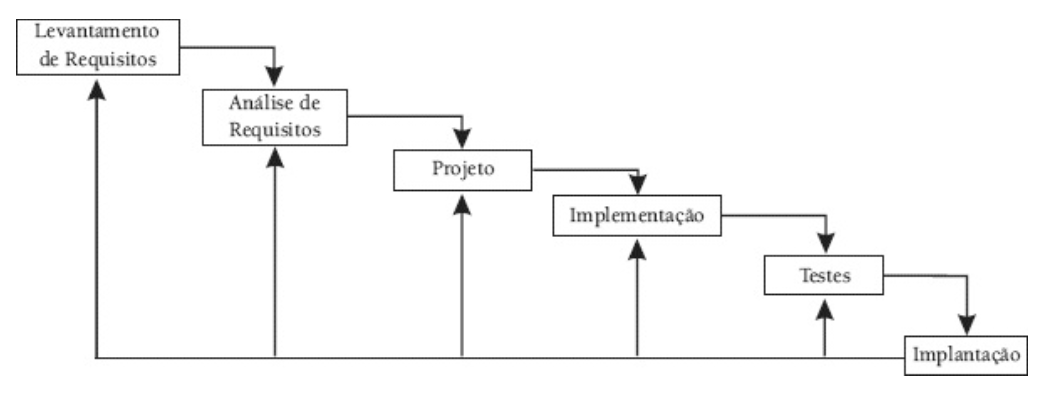
\includegraphics[scale=0.4]{imagens/cascata.png}
	\caption{Modelo cascata \cite{bezerra2016principios}}
	\label{fig:modelo-cascata}
\end{figure}

\subsubsection{O modelo de processo de software iterativo e incremental}

Segundo \citeonline{bezerra2016principios} , o modelo de processo de software incremental e iterativo foi proposto como uma resposta aos problemas encontrados no modelo em cascata. Um processo de desenvolvimento utilizando essa abordagem divide o desenvolvimento de um produto de software em ciclos. Em cada ciclo dessa etapa podem ser identificadas as fases de análise, projeto, implementação e testes. Essa característica contrasta com a abordagem clássica, na qual as fases de análise, projeto, implementação e testes são realizadas uma única vez.

\begin{figure}[H]
	\centering
	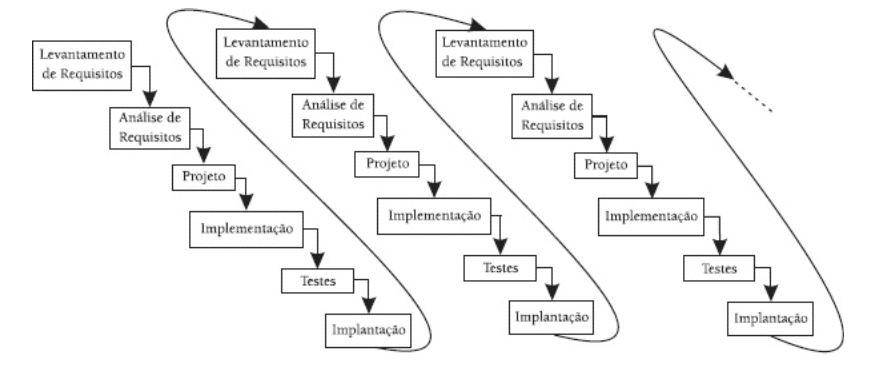
\includegraphics[scale=0.5]{imagens/interativo-incremental.png}
	\caption{No processo incremental e iterativo, cada iteração é uma minicascata. \cite{bezerra2016principios}}
	\label{fig:interativo-incremental}
\end{figure}

\subsubsection{Modelos de processo evolucionário}

Software, assim como todos sistemas complexos, evolui ao longo do tempo. Conforme o de- senvolvimento do projeto avança, as necessidades de negócio e de produto mudam frequente- mente, tornando inadequado seguir um planejamento em linha reta de um produto final \cite{pressman2016engenharia}. Assim, faz-se necessário um modelo de processo que tenha sido projetado especificamente para desenvolver um produto que evolua ao longo do tempo.

Modelos evolucionários são iterativos. Apresentam características que possibilitam desen- volver versões cada vez mais completas do software. Nos parágrafos seguintes, são apresenta- dos dois modelos comuns em processos evolucionários \cite{pressman2016engenharia}.

\subsubsubsection{Prototipação}

Na sua forma ideal, o protótipo atua como um mecanismo para identificar os requisitos do software. Caso seja necessário desenvolver um protótipo operacional, pode-se utilizar partes de programas existentes ou aplicar ferramentas (por exemplo, geradores de relatórios e gerencia- dores de janelas) que possibilitem gerar rapidamente tais programas operacionais.

O protótipo pode servir como “o primeiro sistema”. Aquele que Brooks recomenda que se jogue fora. Porém, essa pode ser uma visão idealizada. Embora alguns protótipos sejam cons- truídos como “descartáveis”, outros são evolucionários, no sentido de que evoluem lentamente até se transformar no sistema real \cite{pressman2016engenharia}.

\begin{figure}[H]
	\centering
	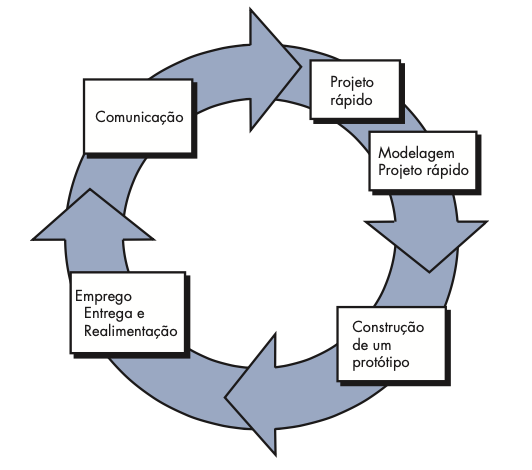
\includegraphics[scale=0.4]{imagens/prototipacao.png}
	\caption{Modelo Prototipação \cite{pressman2016engenharia}}
	\label{fig:prototipacao}
\end{figure}


\subsubsubsection{Modelo Espiral}

É um modelo de processo de software evolucionário que acopla a natureza iterativa da prototi- pação com os aspectos sistemáticos e controlados do modelo cascata. Fornece potencial para o rápido desenvolvimento de versões cada vez mais completas do software \cite{pressman2016engenharia}.

\begin{figure}[H]
	\centering
	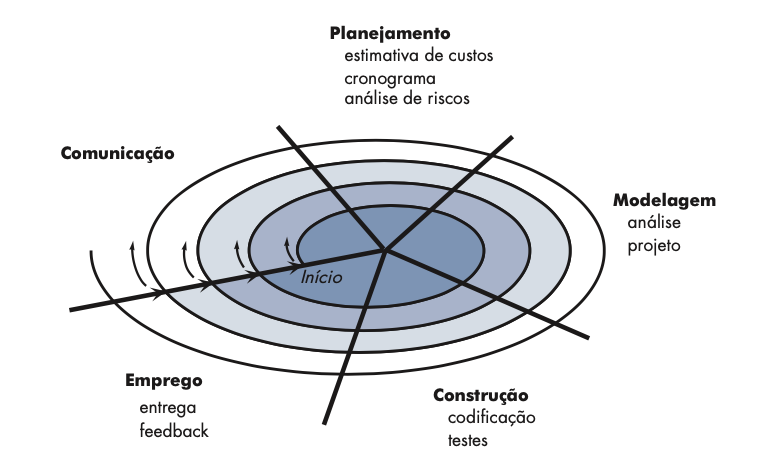
\includegraphics[scale=0.4]{imagens/espiral.png}
	\caption{Modelo em espiral \cite{pressman2016engenharia}}
	\label{fig:espiral}
\end{figure}

O modelo espiral é uma abordagem realista para o desenvolvimento de sistemas e de software em larga escala. Pelo fato de o software evoluir à medida que o processo avança, o desenvolvedor e o cliente compreendem e reagem melhor aos riscos\footnote{Risco pode ser entendido como a avaliação da probabilidade de um perigo ocorrer e no cálculo de seu possível impacto e prejuízo para a corporação.} em cada nível evolucionário.



